\documentclass{beamer}
\usepackage[utf8]{inputenc}
\usepackage[T2A]{fontenc}
\usepackage[english,russian]{babel}

\usetheme{Madrid}
\usecolortheme{default}

\usepackage{dejavu}

%------------------------------------------------------------
%This block of code defines the information to appear in the
%Title page
\title[Продвинутый 3D renderer] %optional
{Продвинутый 3D renderer}

\subtitle{Программный проект}

\author[Смородинов Александр] % (optional)
{Смородинов Александр, БПМИ196\\
	\text{}\\
Научный руководитель: \\
доцент, кандидат физико-математических наук, \\
Трушин Дмитрий Витальевич}

\institute[ВШЭ] % (optional)
{
	Факультет Компьютерных Наук\\
	НИУ ВШЭ (Москва)
}

\date[Июнь 2022] % (optional)
{Июнь 2022}

%End of title page configuration block
%------------------------------------------------------------



%------------------------------------------------------------
%The next block of commands puts the table of contents at the 
%beginning of each section and highlights the current section:

\AtBeginSection[]
{
	\begin{frame}
		\frametitle{Содержание}
		\tableofcontents[currentsection]
	\end{frame}
}
%------------------------------------------------------------

\newcommand{\pl}{\item[\textcolor{green}{+}]}
\newcommand{\mi}{\item[\textcolor{red}{$-$}]}

\begin{document}
	
	%The next statement creates the title page.
	\frame{\titlepage}
	
	
	%---------------------------------------------------------
	%This block of code is for the table of contents after
	%the title page
	\begin{frame}
		\frametitle{Содержание}
		\tableofcontents
	\end{frame}
	%---------------------------------------------------------
	
	
	\section{Предметная область}
	
	\begin{frame}
		\frametitle{3D рендеринг}
		
		\begin{itemize}
			\item<1-> \textbf{3D рендеринг} - преобразование 3D моделей в 2D изображения.
			\item<1-> Для выполнения рендеринга может использоваться: 
			\begin{itemize}
				\item<1-> CPU (программный рендеринг). 
				\item<1-> CPU + GPU (аппаратный рендеринг).
			\end{itemize}
		\end{itemize}
	\end{frame}
	
	\begin{frame}
		\frametitle{Программный vs аппаратный рендеринг}
		
		\begin{itemize}
			\item<1-> Программный рендеринг:
			\begin{itemize}
				\pl<1-> Аппаратная независимость
				\mi<1-> Производительность
			\end{itemize}
			\item<2-> Аппаратный рендеринг:
			\begin{itemize}
				\pl<2-> Производительность
				\mi<2-> Аппаратная независимость
			\end{itemize}
		\end{itemize}
	\end{frame}
	
	\section{Актуальность задачи}
	
	%---------------------------------------------------------
	%Changing visivility of the text
	\begin{frame}
		\frametitle{Актуальность задачи}
		
		\begin{enumerate}
			\item<1-> Востребованность:
			\begin{itemize}
				\item<1-> 3D рендеринг широко распространен, используется в 3D моделировании и анимации, в 3D и VR симуляциях, в компьютерных играх. Данная область относительно молодая и постоянно развивается.
				\item<1-> Программный рендеринг применяется в случаях, когда важна аппаратная независимость и производительность не является критическим требованием.
			\end{itemize}
			\item<2-> Нерешённость:
			\begin{itemize}
				\item<2-> Как будет показано далее, в открытом доступе \textit{программных} рендереров, реализующих \textbf{продвинутые} алгоритмы отрисовки, достаточно мало.
			\end{itemize}
		\end{enumerate}
	\end{frame}
	
	\section{Цель и задачи}
	\begin{frame}
		\frametitle{Цель и задачи}
		
		\begin{enumerate}
			\item<1-> Цель:
			\begin{itemize}
				\item<1-> Изучить и реализовать \textit{продвинутые} алгоритмы отрисовки и таким образом \textit{дополнить} и \textit{улучшить} базовый 3D рендерер, реализованный в прошлом году.
			\end{itemize}
			\item<2-> Основные задачи:
			\begin{itemize}
				\item<2-> Изучить различные продвинутые алгоритмы отрисовки.
				\item<2-> Реализовать данные алгоритмы и интегрировать их в существующую реализацию 3D рендерера.
				\item<2-> Протестировать реализованные алгоритмы.
			\end{itemize}
			\item<3-> Дополнительные задачи:
			\begin{itemize}
				\item<3-> Рефакторинг и улучшение качества кода 3D рендерера.
				\item<3-> Оптимизация, улучшение производительности.
				\item<3-> Написание сопроводительной документации, описание деталей реализации, изложение теоретических основ алгоритмов.
			\end{itemize}
		\end{enumerate}
	\end{frame}
	
	\begin{frame}
		\frametitle{Формальная постановка задачи}

		\begin{enumerate}
			\item<1-> Задача - реализовать следующие алгоритмы:
			\begin{itemize}
				\item<1-> Normal mapping, parallax mapping, HDR, tone mapping, gamma correction, bloom, рендеринг полупрозрачных объектов (blending), shadow mapping, deferred shading, SSAO. 
			\end{itemize}
			\item<2-> Результат проекта - интерактивное приложение, доступное на ОС windows / linux, в котором пользователь может:
			\begin{itemize}
				\item<2-> Просматривать различные 3D сцены, управляя камерой с клавиатуры.
				\item<2-> Настраивать параметры сцены.
				\item<2-> Открывать и добавлять в сцену 3D объекты, сохранённые в различных форматах (поддерживаются 3D модели в формате wavefront obj).
			\end{itemize}
		\end{enumerate}
	\end{frame}
	
	\begin{frame}
		\frametitle{Нефункциональные требования}
	
		\begin{itemize}
			\item<1-> Язык программирования - C++ (стандарт C++17).
			\item<1-> Используемые библиотеки (статическая линковка):
			\begin{itemize}
				\item<1-> glm 0.9.9
				\item<1-> SFML 2.5.1
				\item<1-> ImGui v1.83
			\end{itemize}
			\item<1-> Система контроля версий - git. Репозиторий: \\ {\scriptsize \url{https://github.com/asmorodinov/3d-renderer-from-scratch/tree/dev}}.
			\item<1-> Линтер/форматтер - clang format, настройки основаны на google codestyle.
			\item<1-> Для сборки проекта используется IDE Microsoft Visual Studio 2019.
		\end{itemize}
	\end{frame}
	
	%---------------------------------------------------------
	
	\section{Обзор существующих решений}
	\begin{frame}
		\frametitle{Обзор существующих решений}
		
		\begin{itemize}
			\item<1-> Mesa - {\scriptsize \url{https://www.mesa3d.org/}}.
			\begin{itemize}
				\item<1-> Реализация набора видеодрайверов для основных графических API.
				\item<1-> Программная реализация OpenGL 3.1.
				\item<1-> Широкое распространение на устройствах с GNU/Linux, *BSD и др., в качестве основы графического стека. 
			\end{itemize}
			\item<2-> Другие аналоги - самые популярные github репозитории (по количеству звёзд) с темой software rendering:
			\begin{itemize}
				\item<2-> ssloy/tinyrenderer, zauonlok/renderer, kosua20/herebedragons, skywind3000/mini3d, ssloy/tinyraycaster, skywind3000/RenderHelp, Angelo1211/SoftwareRenderer, martinResearch/DEODR
				\item<2-> bytecode77/fastpix3d, Dawoodoz/DFPSR
				\item<2-> Ни один из перечисленных выше аналогов не реализует \textit{все} \textit{продвинутые} алгоритмы, указанные на прошлых слайдах. Хотя все аналоги достаточно интересны (особенно последние два), и немного более подробно я их описывал в отчёте.
			\end{itemize}
		\end{itemize}
	\end{frame}

\section{\textit{Краткое} описание реализованных алгоритмов}

\begin{frame}
	\frametitle{HDR}
	
	\begin{itemize}
		\item<1-> \textbf{LDR} - все компоненты цвета лежат в ограниченном диапазоне ($[0, 1]$, или $0, \ldots, 255$).
		
		\item<1-> \textbf{HDR} - компоненты цвета ограничены по величине только максимальным значением типа (например \textit{float32}).
		
		\item<1-> Из HDR в LDR цвет преобразуется с помощью tone mapping.
		
	\end{itemize}
\end{frame}

\begin{frame}
	\frametitle{Bloom}
	
	\begin{itemize}
		\item<1-> Отрисовываем сцену в HDR буфер.
		\item<1-> Выделяем из HDR буфера ''яркие'' пиксели.
		\item<1-> Размываем яркие пиксели.
		\item<1-> Прибавляем полученный буфер к исходному.
		\item<1-> Делаем tone mapping.
	\end{itemize}
\end{frame}

\begin{frame}
	\frametitle{Скриншот}
	\begin{center}
		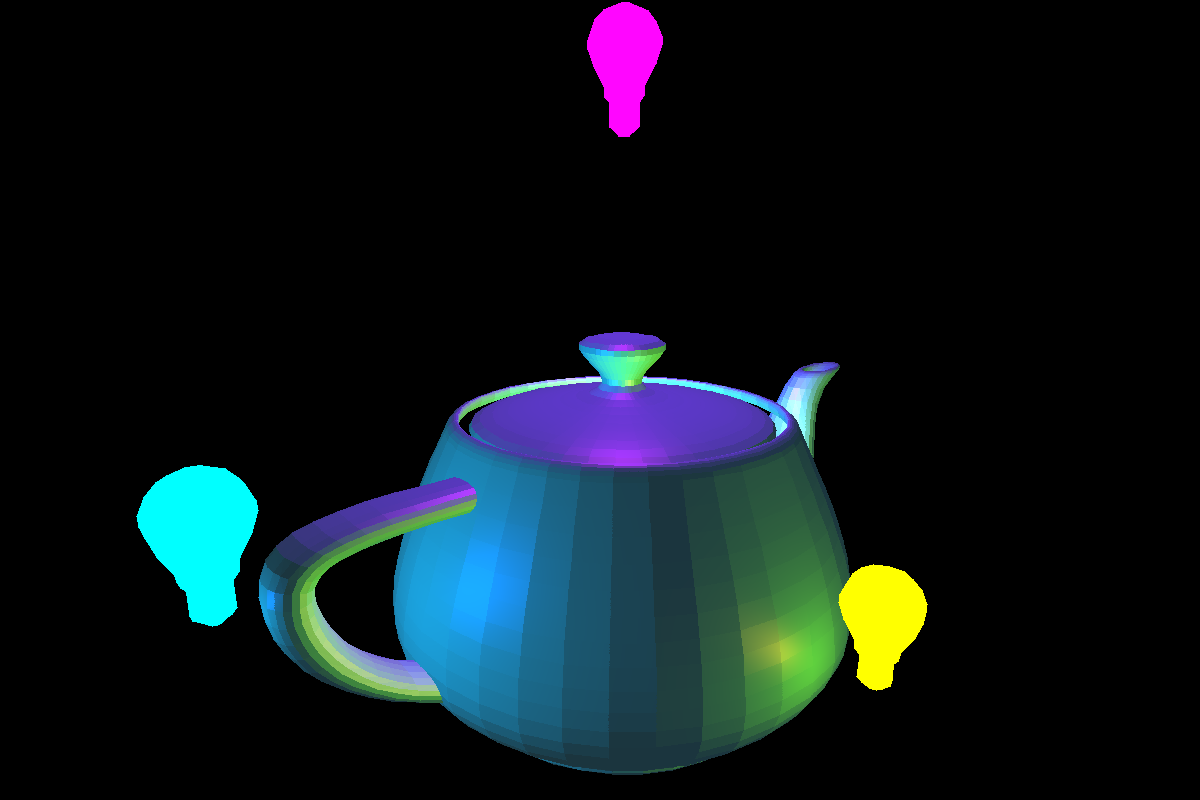
\includegraphics[scale=0.28]{scene.png} 
	\end{center}
\end{frame}

\begin{frame}
	\frametitle{Скриншот}
	\begin{center}
		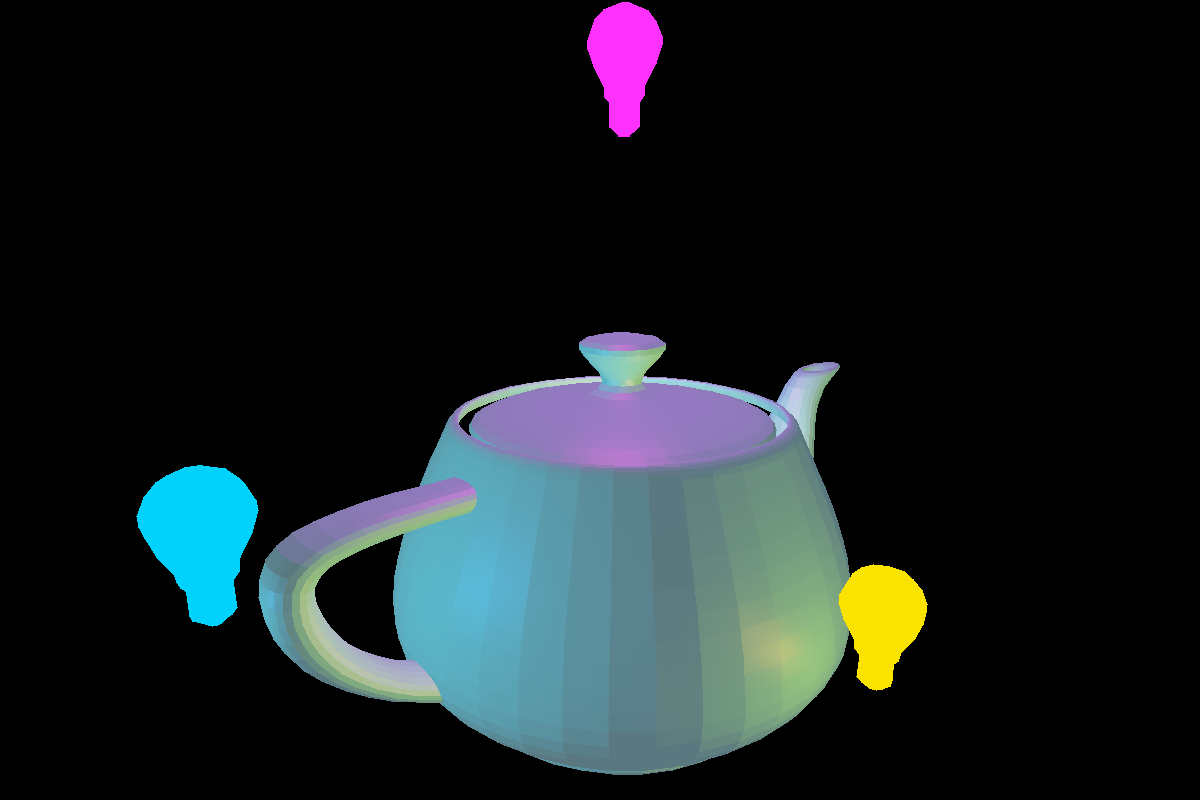
\includegraphics[scale=0.28]{scene2.png} 
	\end{center}
\end{frame}

\begin{frame}
	\frametitle{Скриншот}
	\begin{center}
		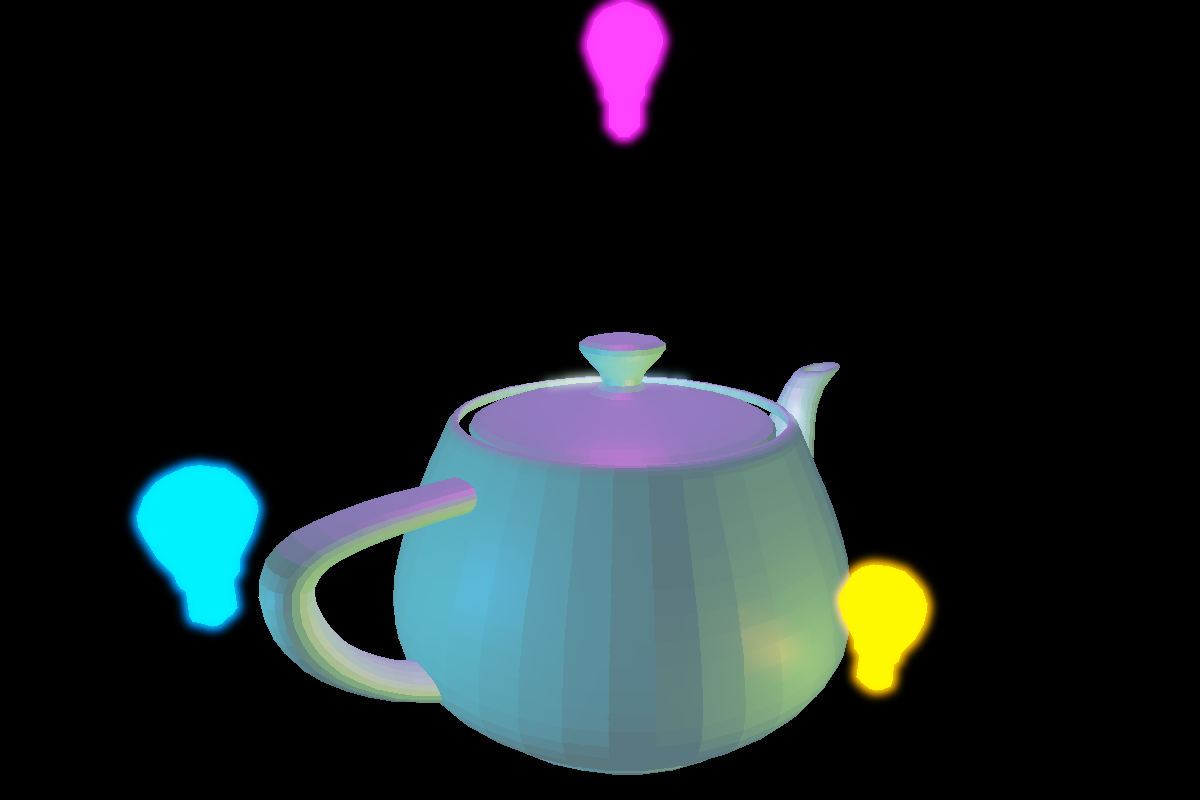
\includegraphics[scale=0.28]{scene3.png} 
	\end{center}
\end{frame}

\begin{frame}
	\frametitle{Отрисовка полупрозрачных объектов, blending}
	
	\begin{itemize}
		\item<1-> Объекты отрисовываются от более дальних к более близким.
		\item<1-> Когда какой-то цвет в буфере (source) перезаписывает цвет уже находящегося в буфере пикселя (destination), вызывается blend функция и результат сохраняется в буфер.
		\item<1-> Blend функция принимает 2 цвета и возвращает результат их ''смешивания'' (тоже цвет). Например $f(s, d) = s * s.a + d * (1 - s.a)$, $s$ - source цвет, $d$ - destination цвет, $x.a$ - значение альфа канала цвета $x$.  
	\end{itemize}
\end{frame}

{
\setbeamercolor{background canvas}{bg=black}
\begin{frame}
	\frametitle{Скриншот}
	\begin{center}
		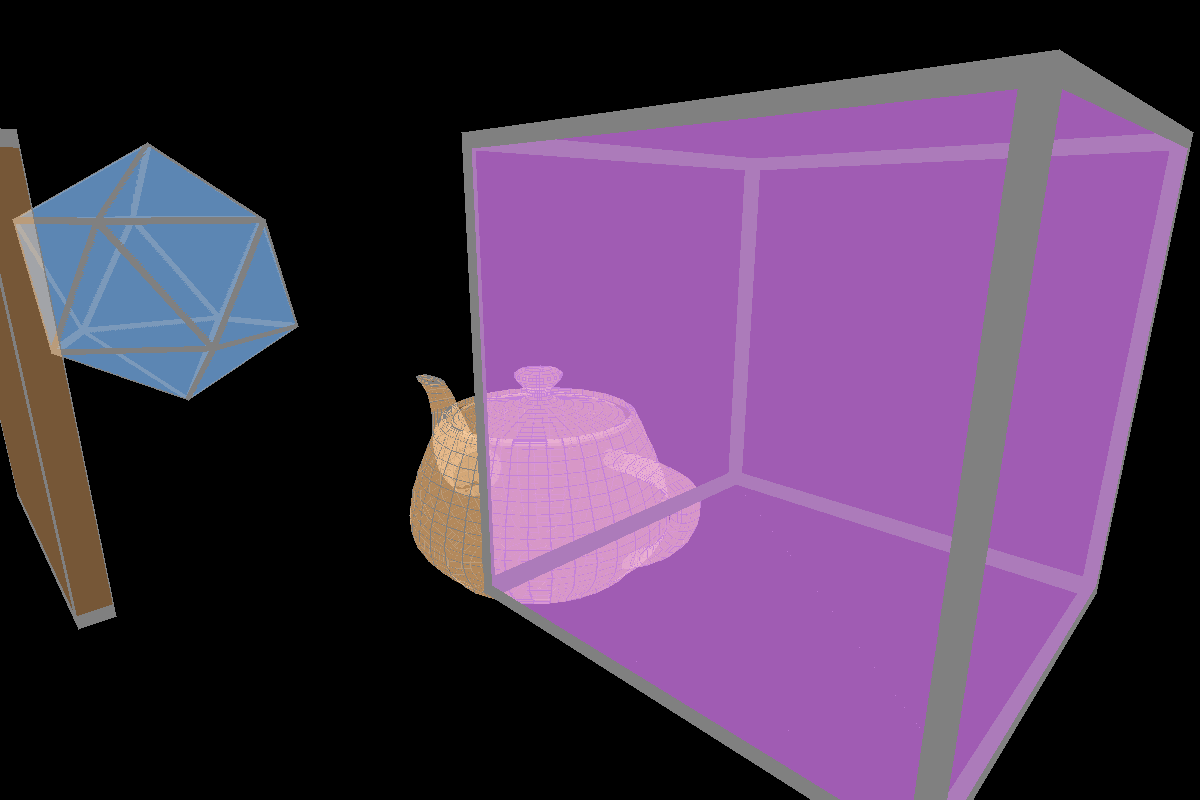
\includegraphics[scale=0.28]{scene4.png} 
	\end{center}
\end{frame}
}

\begin{frame}
	\frametitle{Shadow mapping}
	
	\begin{itemize}
		\item<1-> Сначала отрисовываем сцену с позиции источника света (цвета нас не интересуют, а только буфер глубины).
		\item<1-> С помощью буфера глубины с прошлого шага можно определять, какие фрагменты сцены находятся в тени, а какие - нет.
		\item<1-> Отрисовываем сцену, используя буфер глубины (сейчас уже с цветами).
	\end{itemize}
\end{frame}

\begin{frame}
	\frametitle{Скриншот}
	\begin{center}
		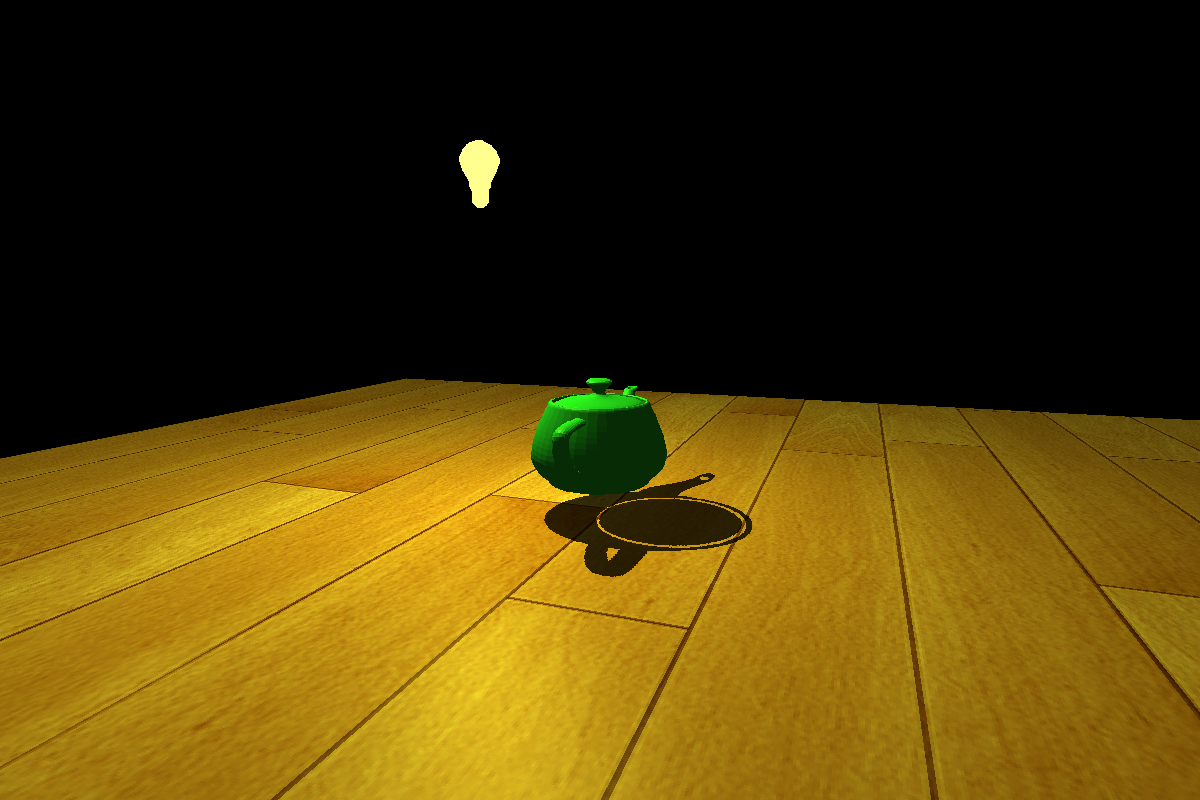
\includegraphics[scale=0.28]{scene5.png} 
	\end{center}
\end{frame}

\begin{frame}
	\frametitle{Normal mapping}
	
	\begin{itemize}
		\item<1-> В шейдерах используем не один вектор нормали для всего примитива (треугольника).
		\item<1-> Вместо этого, мы сначала получаем вектор нормали для текущего фрагмента из карты нормалей (normal map), аналогично тому, как используются обычные текстуры для диффузной составляющей цвета.
		\item<1-> Преобразуем вектор из касательного пространства в пространство мира.
		\item<1-> Далее выполняем стандартные вычисления с полученным вектором (например Blinn-Phong затенение).
	\end{itemize}
\end{frame}

\begin{frame}
	\frametitle{Скриншот}
	\begin{center}
		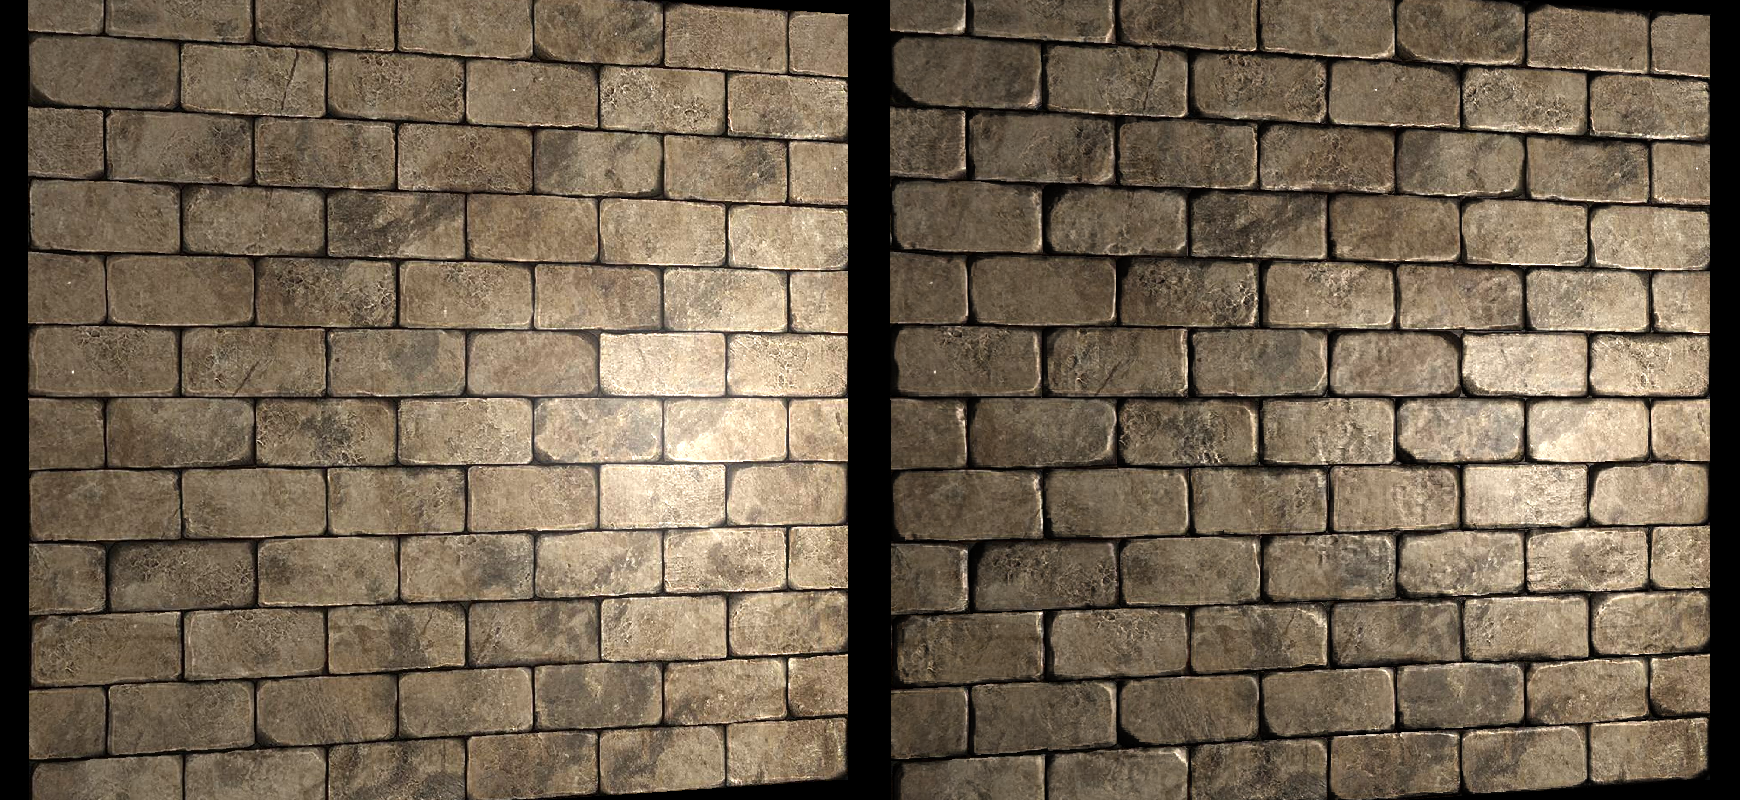
\includegraphics[scale=0.26]{normal.png} 
	\end{center}
\end{frame}

\begin{frame}
	\frametitle{Parallax mapping}
	
	\begin{itemize}
		\item<1-> Идея частично похожа на normal mapping.
		\item<1-> Но для каждого фрагмента теперь задаётся смещение из карты смещения (displacement map).
		\item<1-> По смещению и текстурным координатам фрагмента вычисляются новые текстурные координаты.
		\item<1-> Для всех текстур (normal map, diffuse map) мы используем новые текстурные координаты.
	\end{itemize}
\end{frame}

\begin{frame}
	\frametitle{Скриншот}
	\begin{center}
		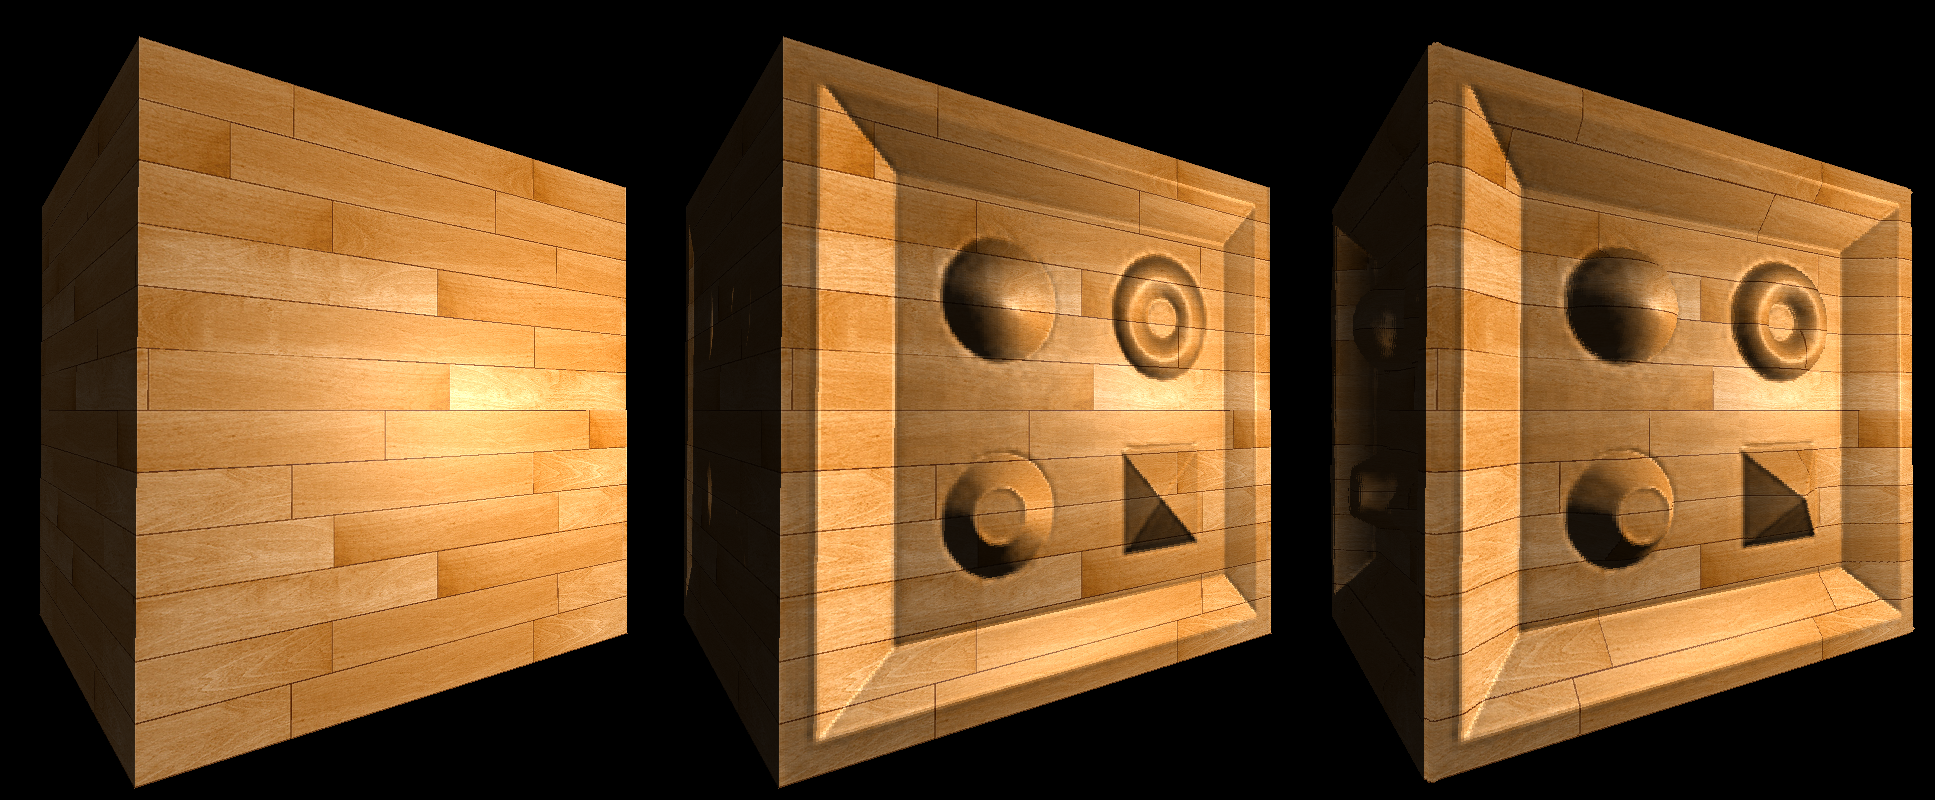
\includegraphics[scale=0.24]{parallax.png} 
	\end{center}
\end{frame}

\begin{frame}
	\frametitle{Отложенное освещение и затенение (deferred shading)}
	
	\begin{itemize}
		\item<1-> Отрисовываем сцену в G-buffer. Элементами G-buffer-а могут например быть вектора позиции фрагмента, диффузной компоненты цвета, нормали и другие.
		\item<1-> Рассчитываем освещение с помощью шейдера, которому на вход подаются элементы G-buffer-а.
	\end{itemize}
\end{frame}


\begin{frame}
	\frametitle{Screen space ambient occlusion (SSAO)}
	
	\begin{itemize}
		\item<1-> SSAO построено на основе отложенного рендеринга.
		\item<1-> SSAO шейдер для каждого фрагмента вычисляет уровень ''окклюзии'' - доли сэмплов, которых не видно с позиции камеры (то есть находящихся за некоторым объектом), рассматриваемых вокруг фрагмента.
		\item<1-> В зависимости от уровня окклюзии меняем величину ambient освещения фрагмента.  
	\end{itemize}
\end{frame}

\begin{frame}
	\frametitle{Скриншот}
	\begin{center}
		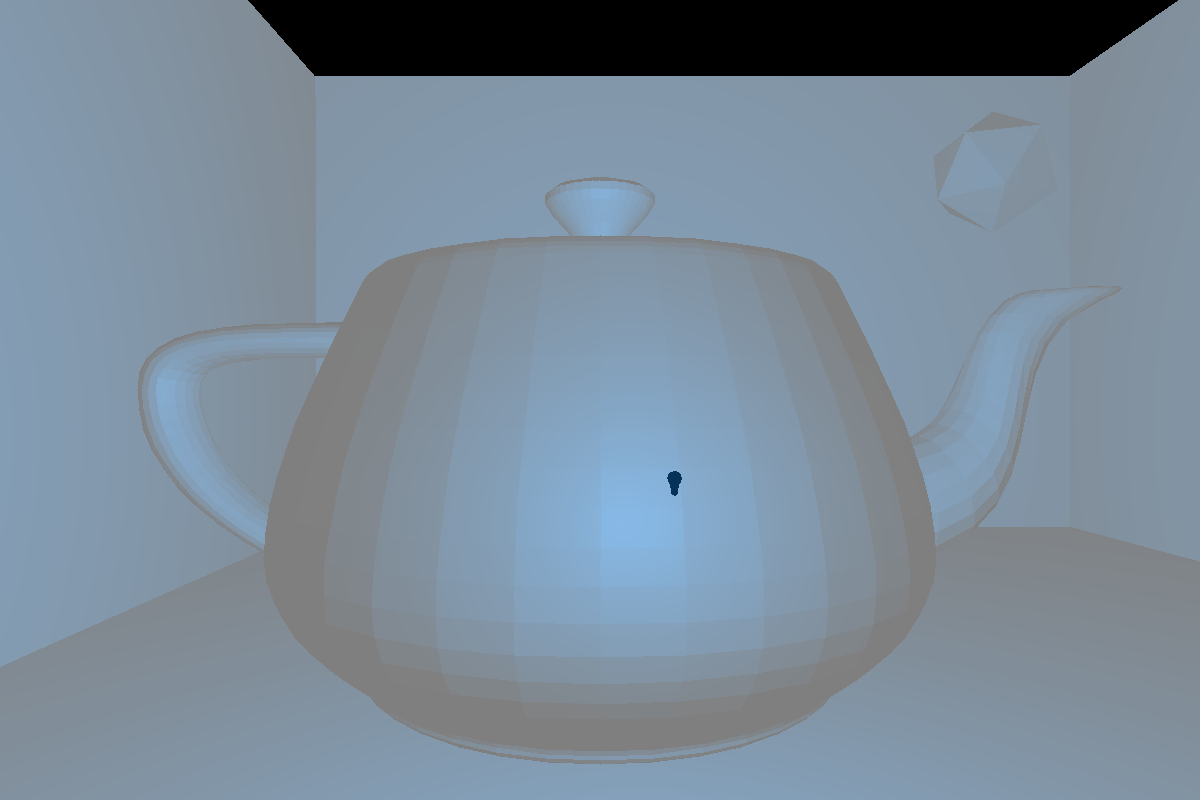
\includegraphics[scale=0.28]{scene6.png} 
	\end{center}
\end{frame}

\begin{frame}
	\frametitle{Скриншот}
	\begin{center}
		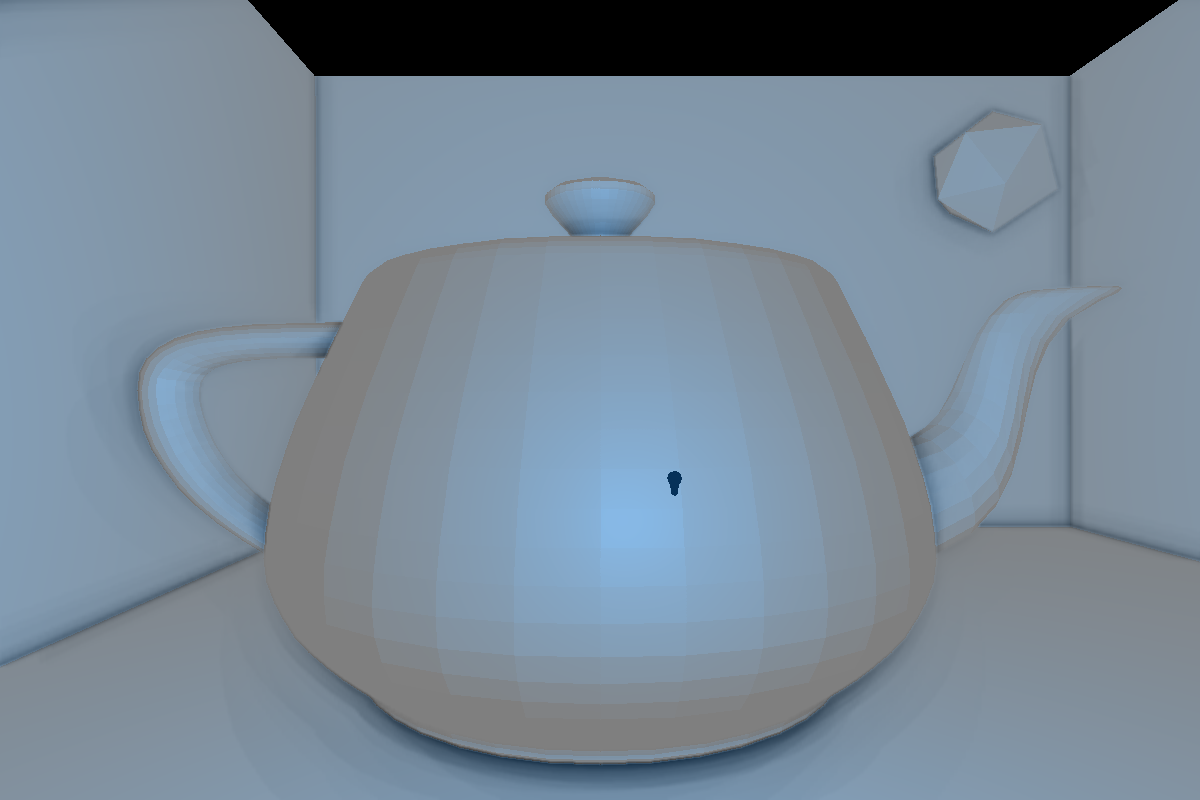
\includegraphics[scale=0.28]{scene7.png} 
	\end{center}
\end{frame}

\section{Детали реализации}
\begin{frame}
	\frametitle{Основные классы}
	
	\begin{itemize}
		\item<1-> \textit{Application}
		\begin{itemize}
			\item<1-> \textit{void run()} - точка входа в event loop.
			\item<1-> Отвечает за координацию своих полей - \textit{SFMLRenderer, UserInterface, CameraControl, std::vector<Scene>}
		\end{itemize}
		\item<1-> \textit{UserInterface} - отвечает за пользовательский интерфейс.
		\item<1-> \textit{CameraControl} - отвечает за обновление позиции и направления камеры (обрабатывает ввод с клавиатуры и мыши).
		\item<1-> \textit{Scene} - хранит в себе вектор объектов и тип пайплайна (строку).
		\item<1-> \textit{Assets} - класс синглтон, хранит текстуры и модели, лениво загружая их по запросу.
		\item<1-> \textit{SFMLRenderer} - обёртка над \textit{Renderer}, умеющая копировать буфер в SFML текстуру, которая отрисовывается на экране.
	\end{itemize}
\end{frame}

\begin{frame}
	\frametitle{Основные классы}
	
	\begin{itemize}
		\item<1-> \textit{Renderer} - хранит в себе различные пайплайны и по переданной сцене определяет, какому пайпалайну отрисовывать её.
		\item<1-> \textit{Pipeline} - есть много классов пайплайнов, каждый из которых отвечает за реализацию конкретного алгоритма отрисовки сцены.
		\item<1-> \textit{Mesh<VertexShader, FragmentShader>} - основной объект сцены, умеет отрисовывать себя в буфере, используя переданные шейдеры.
		\item<1-> \textit{ColorAndDepthBuffer<...>} - набор из двух буферов (глубины и цвета), имеющий ряд полезных вспомогательных функций для работы с ним.
		\item<1-> ...
	\end{itemize}

\end{frame}

\begin{frame}
	\frametitle{Структурная диаграмма классов UML}
	
	\begin{center}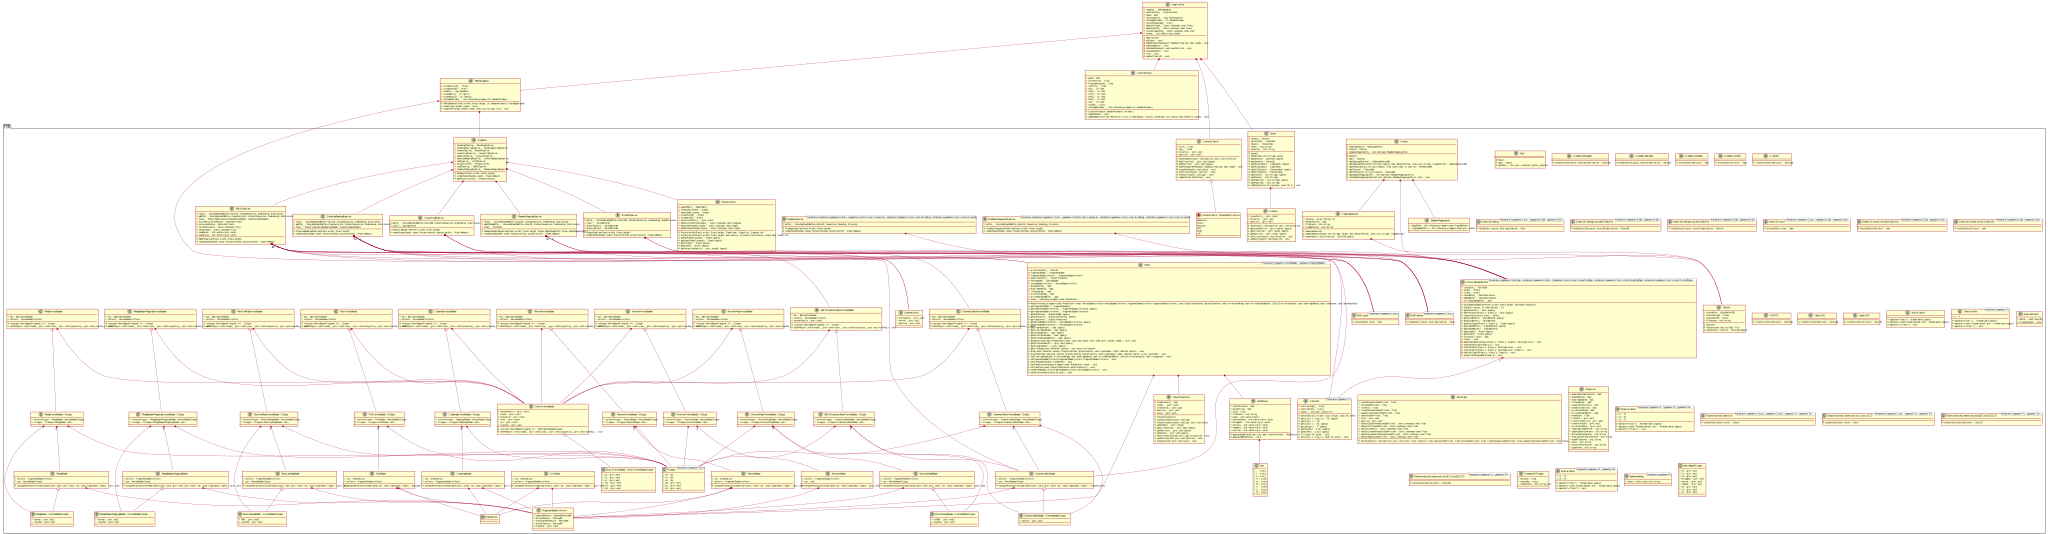
\includegraphics[scale=0.04]{../output.eps}\end{center}
\end{frame}

\section{Тестирование и результаты}
\begin{frame}
	\frametitle{Тесты на производительность}
	
	Intel pentium 4415U, 2.3 GHz, 2 физических (4 виртуальных) ядра, окно в разрешении 1200x800. \\
	\begin{center}\begin{tabular}{|c|c|}
		\hline
		Имя сцены & Время отрисовки кадра, ms \\
		\hline
		bench\_teapot1\_white & 38 \\
		bench\_teapot1\_texture & 44 \\
		bench\_teapot1\_phong & 72 \\
		bench\_teapot1\_phong2 & 85 \\
		bench\_teapot1\_normal & 261 \\
		bench\_teapot1\_disp & 376 \\
		bench\_teapot1\_bloom & 574 \\
		bench\_teapot1\_transparent & 85 \\
		bench\_teapot1\_ssao & 1325 \\
		\hline
	\end{tabular}\end{center}
	
\end{frame}

\begin{frame}
	\frametitle{Тесты на производительность}
	\begin{center}\includegraphics[scale=0.11]{../benchmark.png}\end{center} 
	
\end{frame}

\begin{frame}
	\frametitle{Характеристики ПО}
	\begin{itemize}
		\item<1-> Число строк кода: 2475 в ''.h'' файлах, 2168 в ''.cpp'' файлах. Итого: 4643 строчки кода.
		\item<1-> Объём кода в килобайтах: 147.
		\item<1-> Но необходимо учитывать, что данный проект - это продолжение проекта прошлого года, поэтому не уверен, что по данной статистике можно сделать какие-то определённые выводы.
	\end{itemize} 
\end{frame}

\begin{frame}
	\frametitle{Результаты}
	\begin{itemize}
		\item<1-> Все поставленные задачи были выполнены.
		\item<1-> Главный результат работы - это интерактивное приложение. 
		\item<1-> Были реализованы продвинутые алгоритмы 3D рендеринга: normal mapping, parallax mapping, HDR, bloom, blending (поддержка полупрозрачных объектов), shadow mapping, deferred shading, SSAO.
	\end{itemize}
\end{frame}
	
\begin{frame}
	\frametitle{Fin}
	Спасибо за внимание. \\
	Готов ответить на вопросы.
\end{frame}
	
\end{document}